%!TEX root = ../thesis.tex
\chapter{Numerical investigations\label{sec: numerics}}
We have now established multiple methods for approximating fluid queues which suitable for approximating the performance measures for fluid-fluid queues derived in \cite{bo2014}. In this chapter we numerically investigate various aspects of the approximation schemes. Throughout, we compare the QBD-RAP scheme (from Chapters~\ref{sec: conv} and \ref{sec: construction and modelling}), the discontinuous Galerkin method (without limiters or filtering of the solution) (as decribed in Chapter~\ref{ch:galerkin}), and the spatially-coherent uniformisation as described in \cite{bo2013} (which we will refere to a just the \emph{uniformisation scheme}). Recall that the uniformisation scheme is equivalent to a discontinuous Galerking scheme with a constant basis function in each cell, which is also equivalent to the finite-volume method with an upwind flux. Like the QBD-RAP scheme, due to its stochastic interpretation, the uniformisation scheme is positivity preserving. 


Where appropriate, we also compare the above methods with the discontinuous Galerkin method with a slope-limiter implemented, which avoids oscilations and negative solutions. However, recall that, in the context of approximating operators of fluid-fluid queues with these schemes, slope-limiting is not possible, and even when slope limiting is possible, the resultant approximation is at best linear around discontinuities. 

The main focus of our numerical experiments is on the convergence properties as the number of basis functions is increased. For discontinuous Galerkin method, this means increasing the number of basis functions used to approximate the solution within each cell. For the QBD-RAP scheme, this means increasing the order of the CME distribution used to constrcut the scheme. For the uniformisation scheme, this means dividing each cell into smaller sub-cells over which we approximate the solution. As such, each approximation scheme leads to approximations which are matrices of the same size (although not necessarily the same number of non-zero components). For example, if we use 3 basis functions in the discontinuous Galerkin method, we approximate the solution by a quadratic on each cell; the comparable QBD-RAP scheme is to use a CME of order 3; and the comparable uniformisation scheme is to divide each cell into 3 sub-cells of width \(\Delta/3\). 

To keep the content of this chapter contained, we do not investigate the performance of the schemes as the cell sizes are decreased, other than for the uniformisation scheme. As such, for each numerical experiment, we keep the cell size fixed. As part of deriving a discontinuous Galerkin scheme, one needs to choose the \emph{numerical flux} which is used to approximate the transition of density from one cell to the next and link all the cells together. We investigate schemes with an upwind flux only.
We do not investigate the stability of the schemes with respect to the step-size of the time-integration or time-integration scheme (where required). Instead, we fix the time-integration step size for each numerical experiment at a suitably small value so as to obey a certain stability criterion (a CFL-like condition, REFs, appendix?). For schemes which require us to integrate over time we always implement the strong stability preserving Runge-Kutta method of order 4 with 5 stages (see appendix and REF). This scheme claims to introduce no more oscilations into the solution as we integrate over time (REFs). Where a slope limiter is implemented, we always implement the \emph{Generalised MUSCL} limiter (REF and Appendix). We do not investigate filtering for the DG scheme (REFs).

The performance of the discontinuous Galerkin method has been well-studied (REFs), and it is well-known that the discontinuous Galerkin method performs remarkably well on problems with smooth solutions (REF). Here, we mostly focus on investigating the numerical performance of the methods on problems with non-smooth solutions, the purpose of this is to emphasise the positivity-preserving properties of the QBD-RAP method. In the stochastic modelling community it is very common to have problems with discontinuous solutions, such as a non-smooth initial conditions (REFs). Even if a fluid-queue is initialised with a smooth initial density, the boundary dynamics may induce transient discontinuities into the problem. There is a very specific set of conditions on the inital density and point masses which must hold for the distribution of the fluid queue to remain smooth as it evolves over time (REFs).Limiting distributions of fluid queues are smooth, however. Further, it is possible that discontinuities are present in the performance measures of fluid-fluid queues. 

As we shall see, if the solution is smooth, then the Galerkin method is highly-effective and displays rapid convergence to the solution as the number polynomial basis functions is increased. However, when the solution is non-smooth oscilations and negative approximations may occur when using the discontinuous Galerkin method, leading to non-sensical solutions. In these cases, the QBD-RAP approximation performs relatively well compared to the other positivity preserving schemes investigated.

% THE STRUCTURE OF THE CHAPTER IS AS FOLLOWS. 

% 1. FUNCTION APPROX./RECONSTRUCTION

% 2. 1d wave eqn

% 3. STATIONARY DISTRIBUTIONS
	% i. SIMPLER
	% ii. MORE COMPLEX
	
% 4. TRANSIENT DISTRIBUTIONS 
	% i. SIMPLER
	% ii. MORE COMPLEX

% 5. HITTING TIMES 
	% i. SIMPLER
	% ii. MORE COMPLEX

% 6. FLUID-FLUID QUEUES

% 7. CONCLUDING REMARKS 

\section{Function approximation/reconstruction}
We start our investigation by looking at how well the methods perform at approximating an initial condition. For the discontinuous Galerkin method, this means projecting the solution on to the set of polynomial functions which define the scheme, then reconstructing the solution. For the spatially-coherent uniformisation scheme, this means looking at the sub-cell averages. For the QBD-RAP scheme, this means computing the initial vector for the approximation, then reconstructing the solutions as described in Section~\ref{sec: closing}. First we investigate three closing vectors we can use for the reconstruction for the QBD-RAP, from which we find that the closing operator in (\ref{eqn:5462}) performs reasonably compared to the others, and we are able to theoretically prove that it converges. Therefore we use this reconstruction method throughout the rest of the chapter.

For this section we consider approximating the initial condition over a single cell of width \(\Delta = 1\). To numerically evaluate integrals arising in the approximation step (inner products and cell averages) we use a simple trapezoidal rule with 10,001 function evaluations. Similarly, we use 10,001 function evaluations to approximate \(L^2\) norms, and also as a finite set of points over which to compute the KS statistics. 

First we briefly investigate the possible choices of closing operators as introduced in Section~\ref{sec: closing}. 

\subsection{QBD-RAP closing operators}
The three closing operators we investgate are the following. The unnormalised closing vector in Equation~(\ref{eqn: alal}). A normalised version of the closing operator in Equation~(\ref{eqn:546}), with the normalised version given by (\ref{eqn: nonlin}). We refer to the closing vector in (\ref{eqn: nonlin}) as the \emph{naive normalised} closing vector. Technically we have not yet proved that the \emph{naive normalised} closing vector leads to a convergent approximation scheme, though it clearly appears to. The third closing vector we investigate is that in Equation~(\ref{eqn:5462}). 

First consider approximating the initial condition with density function \(1(x<0.5)\). In the left-hand side of Figure~\ref{fig: fun 2 ks error qbdrap closing vecs} we plot the Kolmogorov-Smirnov error between the true CDF and the CDF constructed via the QBD-RAP approximation. Interestingly, in this case, the unnormalised error outperforms the other two reconstructions at low orders. It just so happens that, in this case, the error due to truncation of the unnormalised reconstruction destructively interferes with other errors in the reconstruction to cause the error to be lower at low orders for the unnormalised scheme. Figure~\ref{fig: fun 2 ks error qbdrap closing vecs} also shows that the naive normalised and normalised reconstructions perform very similarly -- this is the case throughout much of this subsection. The difference between the naive normalised and normalised reconstructions is how they treat mass in the tail of a matrix exponential distribution (from \(2\Delta\) onward). Intuitively, there should be very little mass in the tail of the distribution as we are using concentrated matrix exponential distributions in the reconstruction. 

If we instead look at the \(L^2\) error between the true PDF and the reconstructions in Figure~\ref{fig: fun 2 ks error qbdrap closing vecs}, then we see that the unnormalised reconstruction performs the poorest. Figure~\ref{fig: fun 2 ks error qbdrap closing vecs} also suggests naive normalised and normalised reconstruction are very similar. 
\begin{figure}
	\centering
	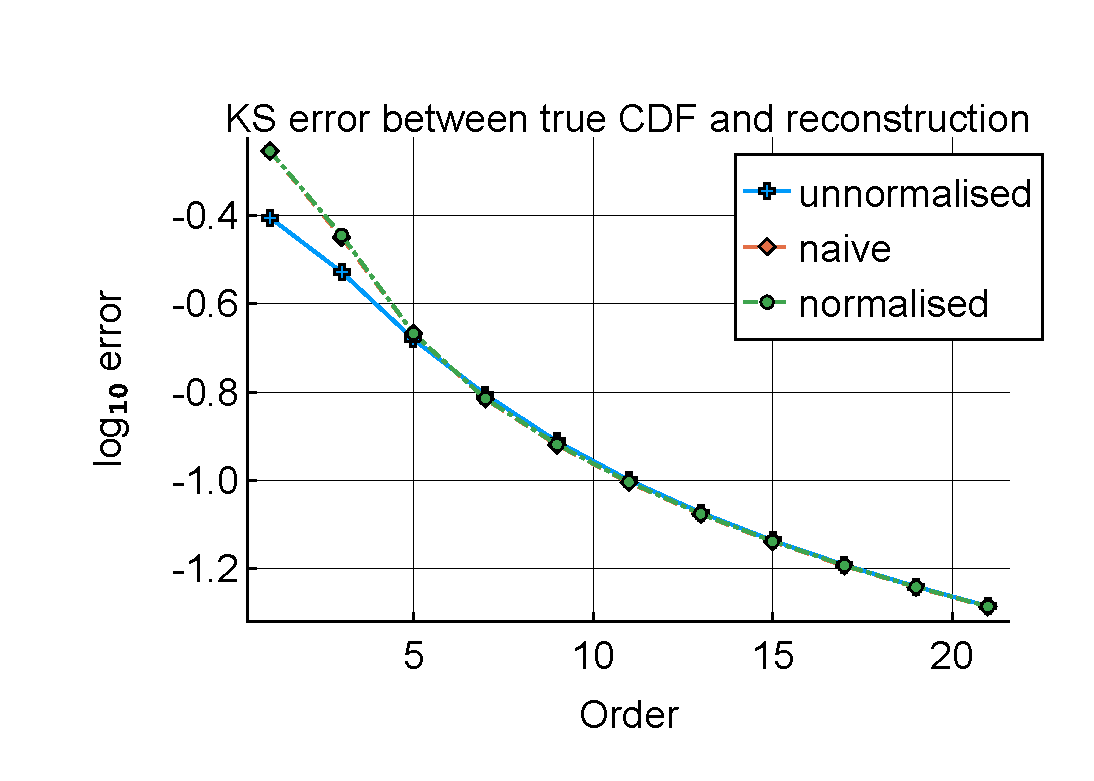
\includegraphics[width=0.5\textwidth,trim={1.25cm 0.8cm 0.25cm 1.25cm},clip]{chapter5/figs/qbdrap_closing_vec/fun2/ks_error_formatted.pdf}%
	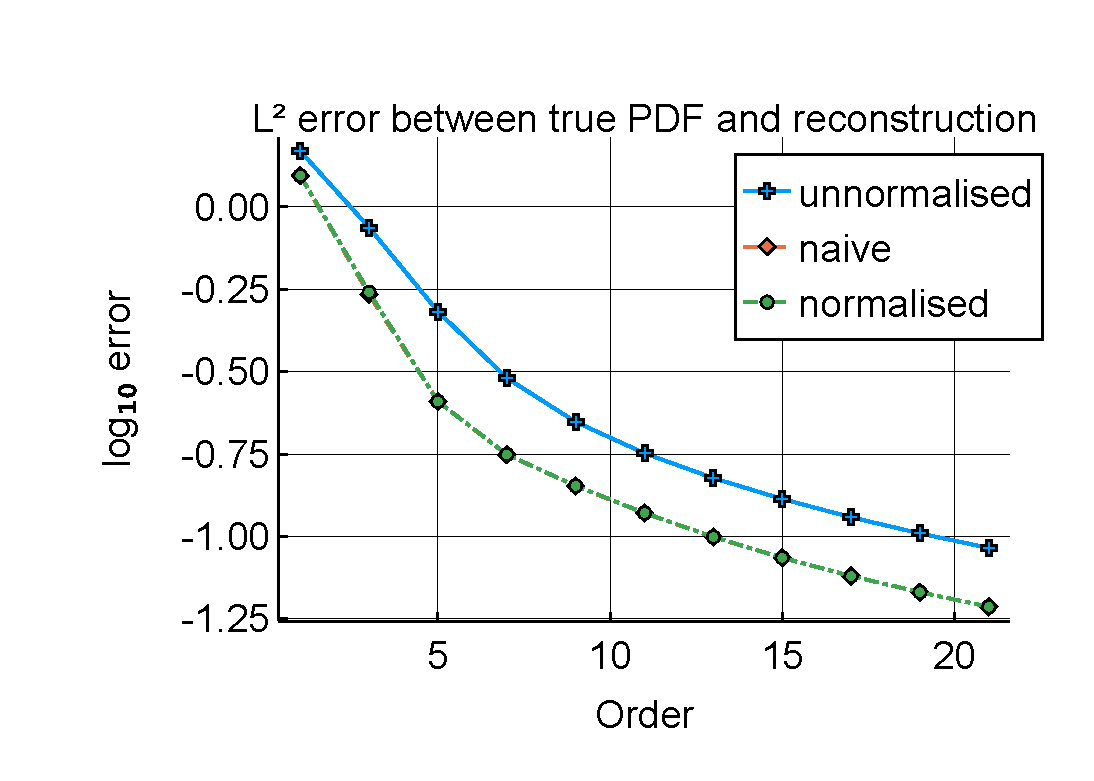
\includegraphics[width=0.5\textwidth,trim={1.25cm 0.8cm 0.25cm 1.25cm},clip]{chapter5/figs/qbdrap_closing_vec/fun2/l2_pdf_error_formatted.pdf}
	\caption{KS error between the true CDF, \(2x1(x<0.5)+1(x\geq 0.5)\), and the approximations (left) and \(L^2\) error between the true PDF, \(2\times 1(x<0.5)\), and the approximations (right) for the three closing vectors considered; unnormalised (blue solid line with crosses), naive normalised (orange dashed line with diamonds) and normalised (green dash-dotted line with circles). The naive normalised (orange) an normalised closing vectors are coincident.}
	\label{fig: fun 2 ks error qbdrap closing vecs}
\end{figure}

Now consider approximating the initial density \(f(x)=1\). Observing Figure~\ref{fig: fun 4 ks error qbdrap closing vecs} of the KS error, and \(L^2\) error between the true initial distribution and the reconstructions, we now see that the normalised reconstructions outperform the unnormalised reconstruction. This suggests that, in this case, the `folding' of closing operator about \(\Delta\) has greatly increased the ability of the reconstruction to approximate this initial distribution. 
\begin{figure}
	\centering
	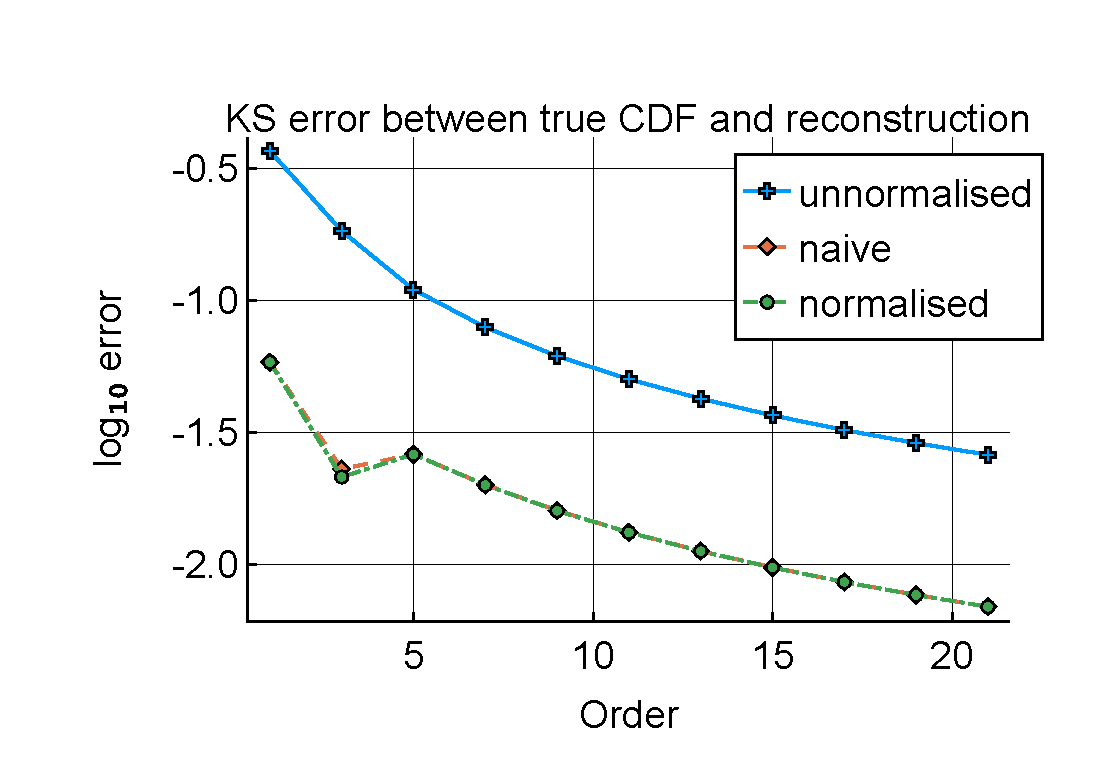
\includegraphics[width=0.5\textwidth,trim={1.25cm 0.8cm 0.25cm 1.25cm},clip]{chapter5/figs/qbdrap_closing_vec/fun4/ks_error_formatted.pdf}%
	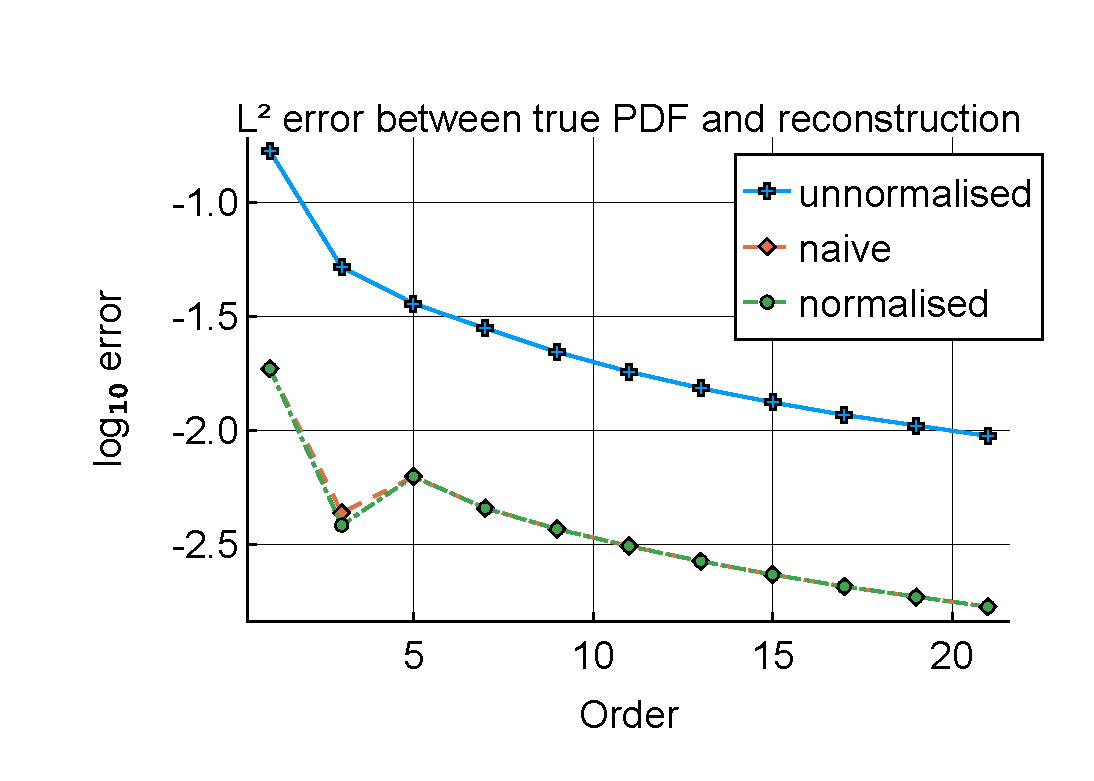
\includegraphics[width=0.5\textwidth,trim={1.25cm 0.8cm 0.25cm 1.25cm},clip]{chapter5/figs/qbdrap_closing_vec/fun4/l2_pdf_error_formatted.pdf}
	\caption{KS error between the true CDF, \(x\), and the approximation (left) and \(L^2\) error between the true PDF and the approximation (right) for the three closing vectors considered; unnormalised (blue solid line with crosses), naive normalised (orange dashed line with diamonds) and normalised (green dash-dotted line with circles). The naive normalised (orange) an normalised closing vectors are coincident.}
	\label{fig: fun 4 ks error qbdrap closing vecs}
\end{figure}

Some insight is gained by looking at Figure~\ref{fig: pdf reconstructed} where we plot the reconstructed PDFs for the unnormalised and normalised closing operators for order 1, 3, 5 and 7, as well as the true PDF. Observing Figure~\ref{fig: pdf reconstructed} notice that the unnormalised reconstruction fails to capture the density at the left of each of the plots and for all orders. This feature is due to a significant amount of mass being lost due to the truncation. In comparison the reconstruction with the normalised closing operator is much better in this region due to the `folding' around \(\Delta\) in the construction of the closing operator. In the reconstruction we also need to allocate the initial condition to a phase with positive rate, or negative rate, so that we can use the appropriate approximation and reconstruction method as discussed in Section~\ref{sec: closing}. Here we suppose that the phase is positive, so the `folding' around \(\Delta\) in the normalised closing operators appears appears at the left of the plots. In general, reconstructions via the unnormalised closing operator typically underestimate the value of the function in this region. 

Figure~\ref{fig: pdf reconstructed} also show that both closing operators do not approximate the initial condition well at the right-hand side of the interval. This is a common feature, and drawback, of the QBD-RAP method. Perhaps there is a different reconstruction method or yet another closing operator which could alleviate this issue. 
\begin{figure}
	\centering
	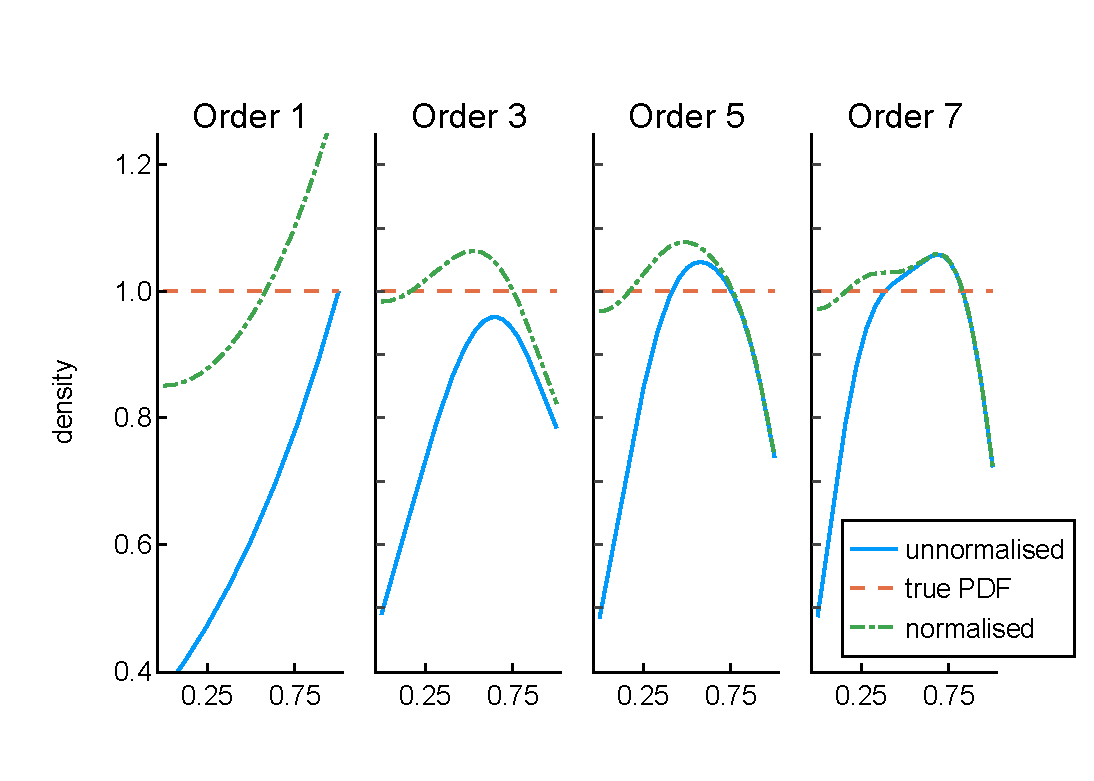
\includegraphics[width=\textwidth]{chapter5/figs/qbdrap_closing_vec/fun4/pdfs_formatted.pdf}
	\caption{Reconstructed PDFs using the unnormalised closing operator (blue solid line), normalised closing operator (green dash-dotted line), for various orders, and the true PDF which is \(f(x)=1\) (orange dashed line).}
	\label{fig: pdf reconstructed}
\end{figure} 

Next we consider approximating the initial distribution with density \(-6x^2+6x\). Observing the left-hand panel of Figure~\ref{fig: fun 6 ks error qbdrap closing vecs}, which plots the KS error against the order of the reconstruction for the three closing operators, we once again see that the reconstruction using the unnormalised closing operator performs the worst, while the performance of the two normalised reconstructions is indistinguishable. However, if we instead look at the right-hand panel of Figure~\ref{fig: fun 6 ks error qbdrap closing vecs}, which plots the \(L^2\) error between the reconstructed PDF and the true PDF, we see that with this metric, then unnormalised closing operator performs better than the two normalised ones for orders 5 and above. 
\begin{figure}
	\centering
	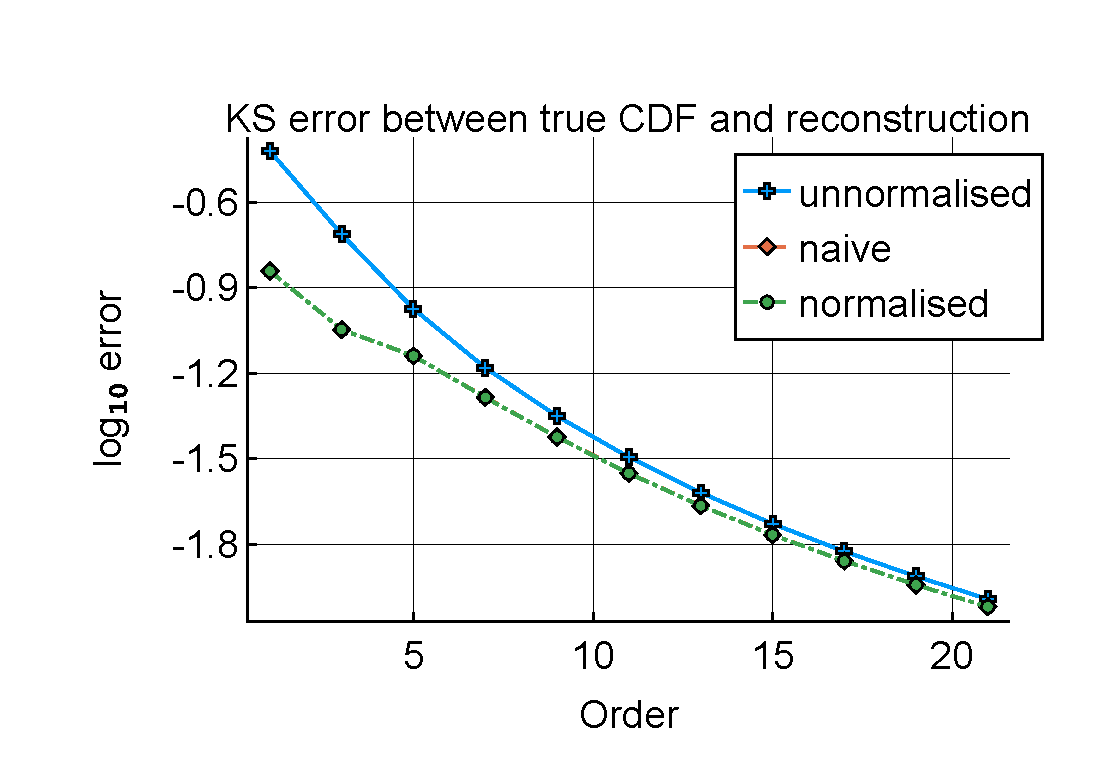
\includegraphics[width=0.5\textwidth,trim={1.25cm 0.8cm 0.25cm 1.25cm},clip]{chapter5/figs/qbdrap_closing_vec/fun6/ks_error_formatted.pdf}%
	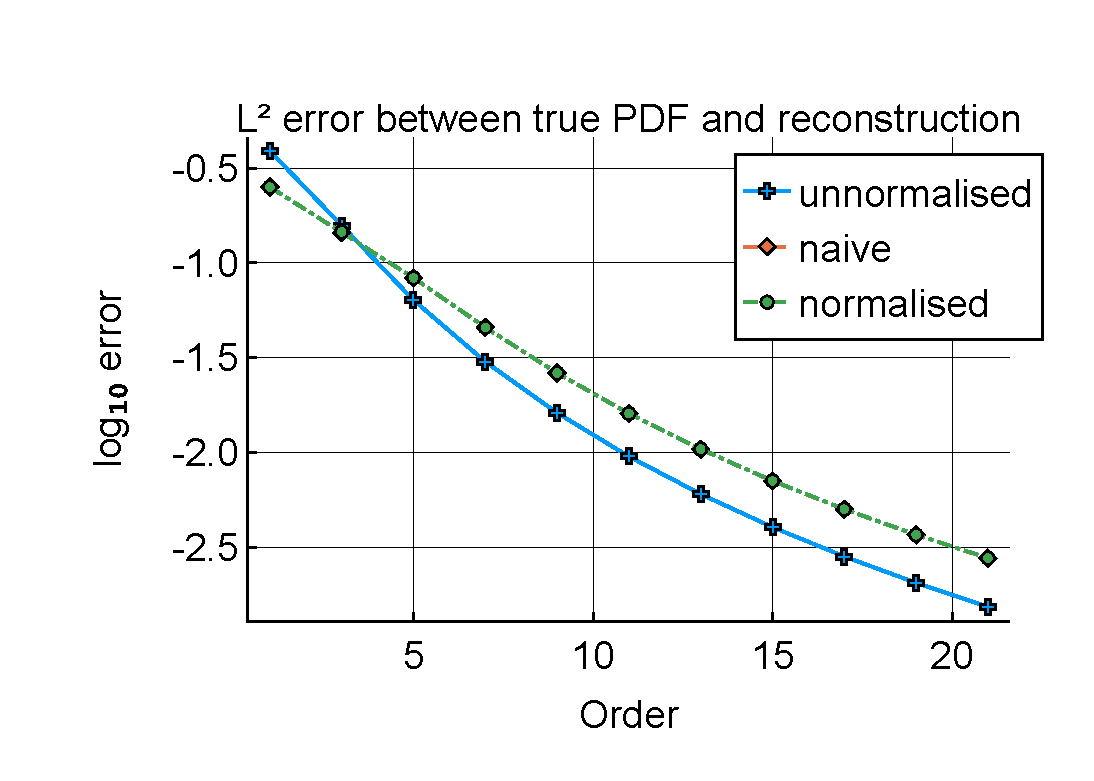
\includegraphics[width=0.5\textwidth,trim={1.25cm 0.8cm 0.25cm 1.25cm},clip]{chapter5/figs/qbdrap_closing_vec/fun6/l2_pdf_error_formatted.pdf}
	\caption{KS error between the true CDF, \(-2x^3+3x^2\), and the approximation (left) and \(L^2\) error between the true PDF \(-6x^2+6x\) and the approximation (right), for the three closing vectors considered; unnormalised (blue solid line with crosses), naive normalised (orange dashed line with diamonds) and normalised (green dash-dotted line with circles). The naive normalised (orange) an normalised closing vectors are coincident.}
	\label{fig: fun 6 ks error qbdrap closing vecs}
\end{figure}

The fact that the unnormalised closing operator outperforms the two normalised ones can be explain, once again, by the fact that, for the normalised operators we have `folded' the ME density function back on itself. In Figure~\ref{fig: pdf reconstructed quadratic} we plot the unnormalised and normalised reconstructions along with the true PDF, \(-6x^2+6x\). In Figure~\ref{fig: pdf reconstructed quadratic} we observe that, at the left of the plot, the normalised reconstructions over estimate the density function in this region, where as the unnormalised reconstruction looks to be doing better. Recall that the `folding' in the normalised closing operator manifest itself as extra mass at the left of these plots compared to the unnormalised reconstructions. 
\begin{figure}
	\centering
	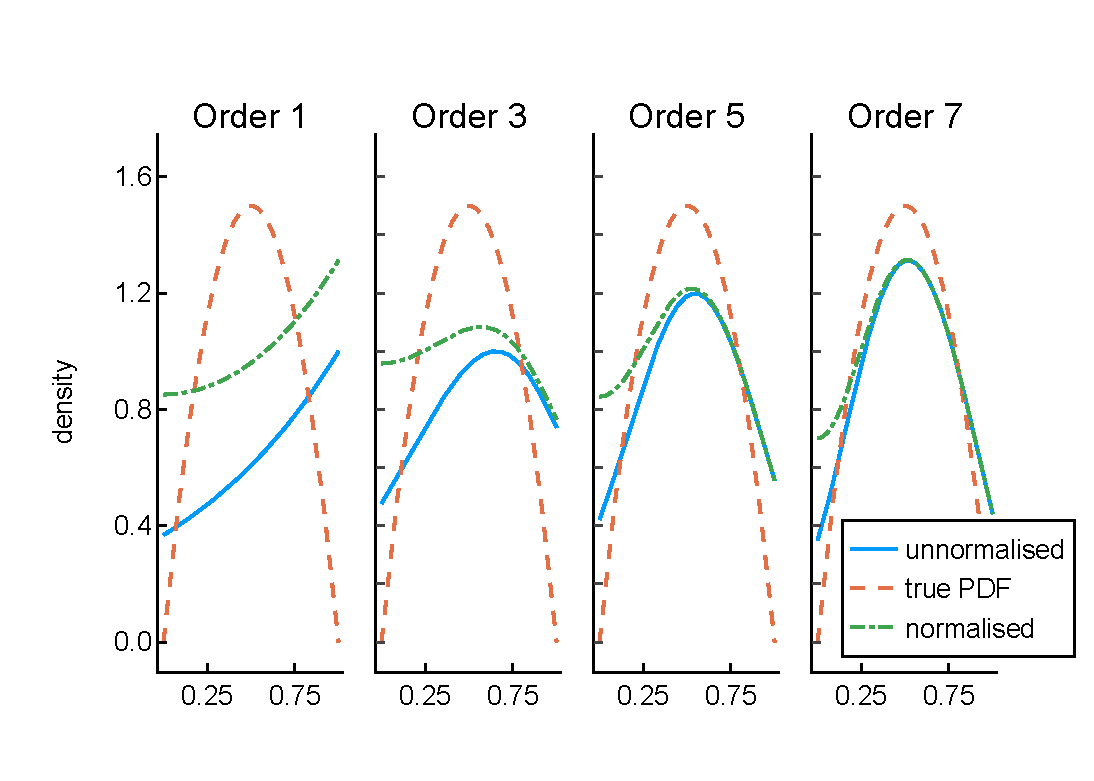
\includegraphics[width=\textwidth]{chapter5/figs/qbdrap_closing_vec/fun6/pdfs_formatted.pdf}
	\caption{Reconstructed PDFs using the unnormalised closing operator (blue solid line), normalised closing operator (green dash-dotted line), for various orders, and the true PDF which is \(f(x)=-6x^2+6x\) (orange dashed line).}
	\label{fig: pdf reconstructed quadratic}
\end{figure} 

Lastly, we consider approximating the initial distribution with PDF \(3e^{-3x}/(1-e^{-3})\). This density function is at a maximum at the left of the region. Considering what we have learnt so far about the unnormalised operator underestimating in this region, we expect that the unnormalised closing operator will perform relatively poorly in this case. Indeed, observing Figures~\ref{fig: fun 7 ks error qbdrap closing vecs} we see that the normalised reconstructions perform relatively well compared to the unnormalised reconstruction as measured by both error metrics (KS statistic and \(L^2\) norm on the PDF). If we observed plots of the PDFs (omitted), we would once again see that this is due to the loss of mass at the left-hand side of the region due to the truncation. 
\begin{figure}
	\centering
	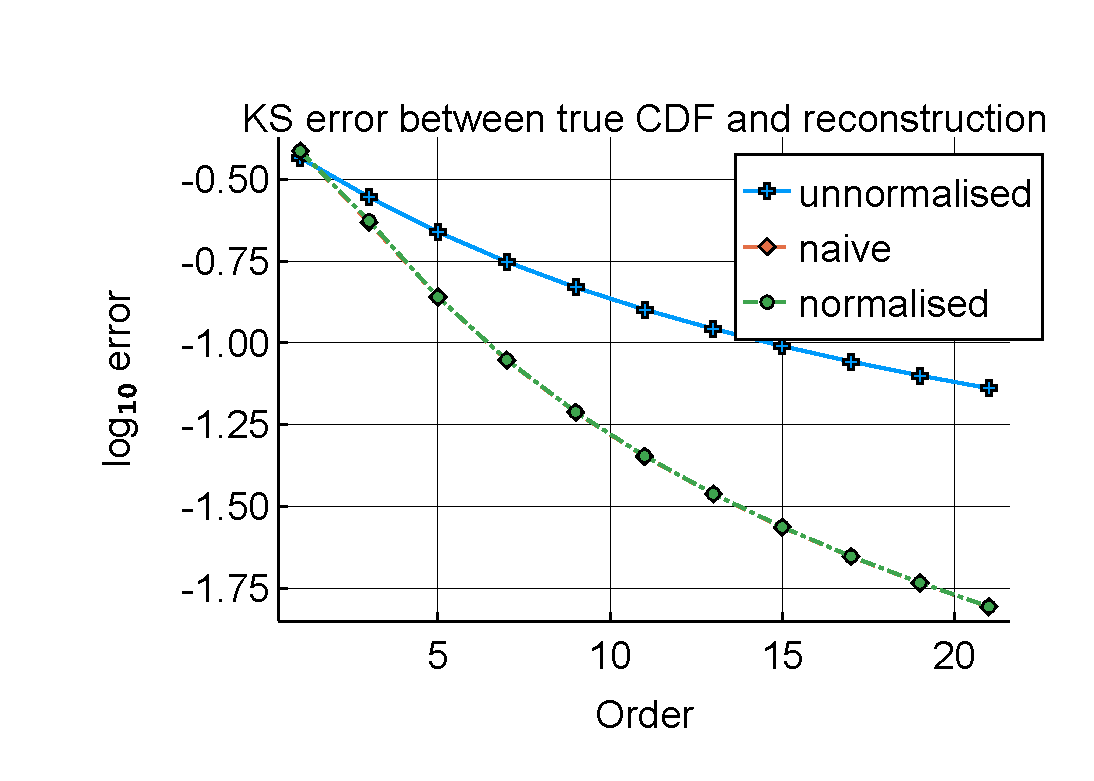
\includegraphics[width=0.5\textwidth,trim={1.25cm 0.8cm 0.25cm 1.25cm},clip]{chapter5/figs/qbdrap_closing_vec/fun7/ks_error_formatted.pdf}%
	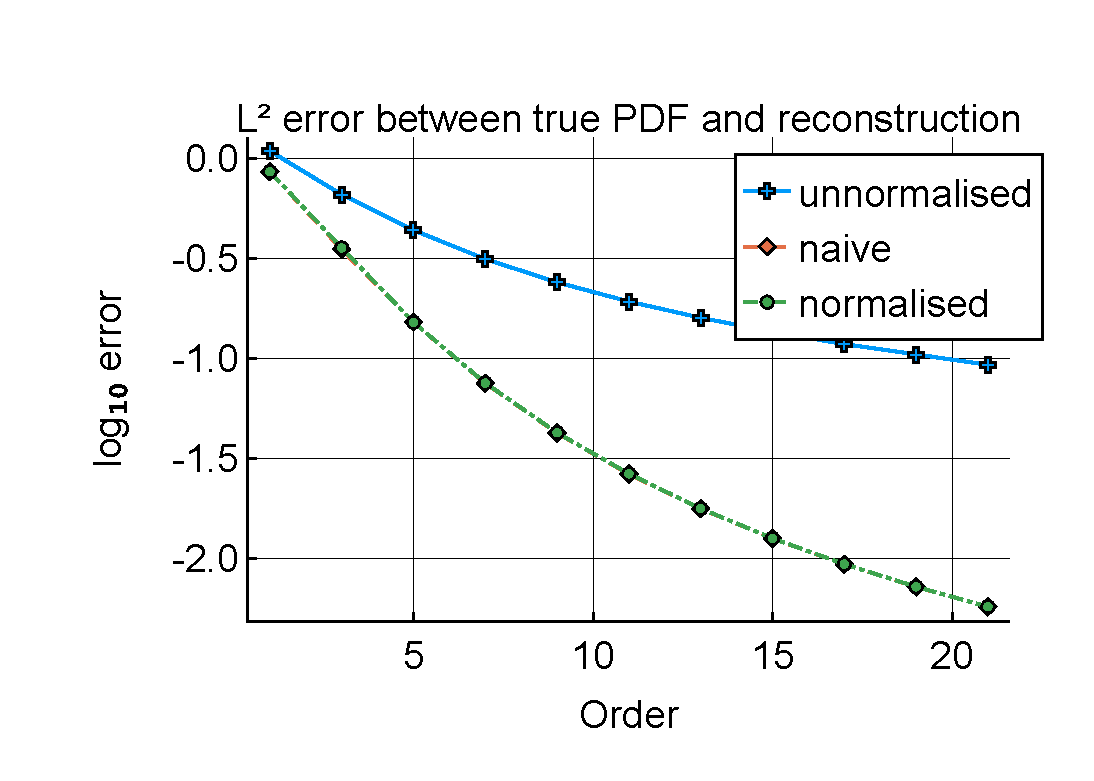
\includegraphics[width=0.5\textwidth,trim={1.25cm 0.8cm 0.25cm 1.25cm},clip]{chapter5/figs/qbdrap_closing_vec/fun7/l2_pdf_error_formatted.pdf}
	\caption{KS error between the true CDF, \((1-e^{-3x})/(1-e^{-3})\), and the approximation (left) and \(L^2\) error between the true PDF and the approximation for the three closing vectors considered; unnormalised (blue solid line with crosses), naive normalised (orange dashed line with diamonds) and normalised (green dash-dotted line with circles). The naive normalised (orange) an normalised closing vectors are coincident.}
	\label{fig: fun 7 ks error qbdrap closing vecs}
\end{figure}

Given the evidence above we choose to use the normalised closing operator to reconstruct solutions. Further, unlike the naive normalised operator, the normalised operator is theoretically justified in that we proved the closing operator leads to a convergent scheme and is linear. 

\subsection{Comparison of methods}
Here we compare the ability of the QBD-RAP, uniformisation, and DG methods to reconstruct initial conditions. 

First we consider the initial condition with CDF \(1(x\geq 0.5)\), that is, a point mass at 0.5. This distribution does not have a PDF so we can compare the CDFs only. In Figure~\ref{fig: fun 1 comp} we plot the KS metric (left) and \(L^1\) metric (right) between the true CDF and the reconstructed approximations. Observing the KS metric, it appears that none of the methods converge and the KS error sits around 0.5. This reflects the fact that convergence in distribution implies pointwise convergence of the CDFs except at points of discontinuity. None of the methods appear to converge at this point. Observing the \(L^1\) error between the true CDF and reconstructed approximation (which is the area between the two CDFs) we now see that the methds appear to show the convergent behaviour we expect. Here, the uniformisation method appears to perform the best, while the QBD-RAP method performs the worst. The rate of convergence of the QBD-RAP method appears to be similar to the rate of convergence of the DG scheme. 

Perhaps it is no surprise that the uniformisation method performs best. In the uniformisation method as we increase the order, we partition the cell \([0,1]\) into smaller sub-cells, and use constant functions on each sub-cell to approximate the function. As such, the uniformisation method can produce a piecewise continous, linear approximation to the CDF. In contrast, both the DG and QBD-RAP methods result in a smooth approximation to the CDF. 
\begin{figure}
	\centering
	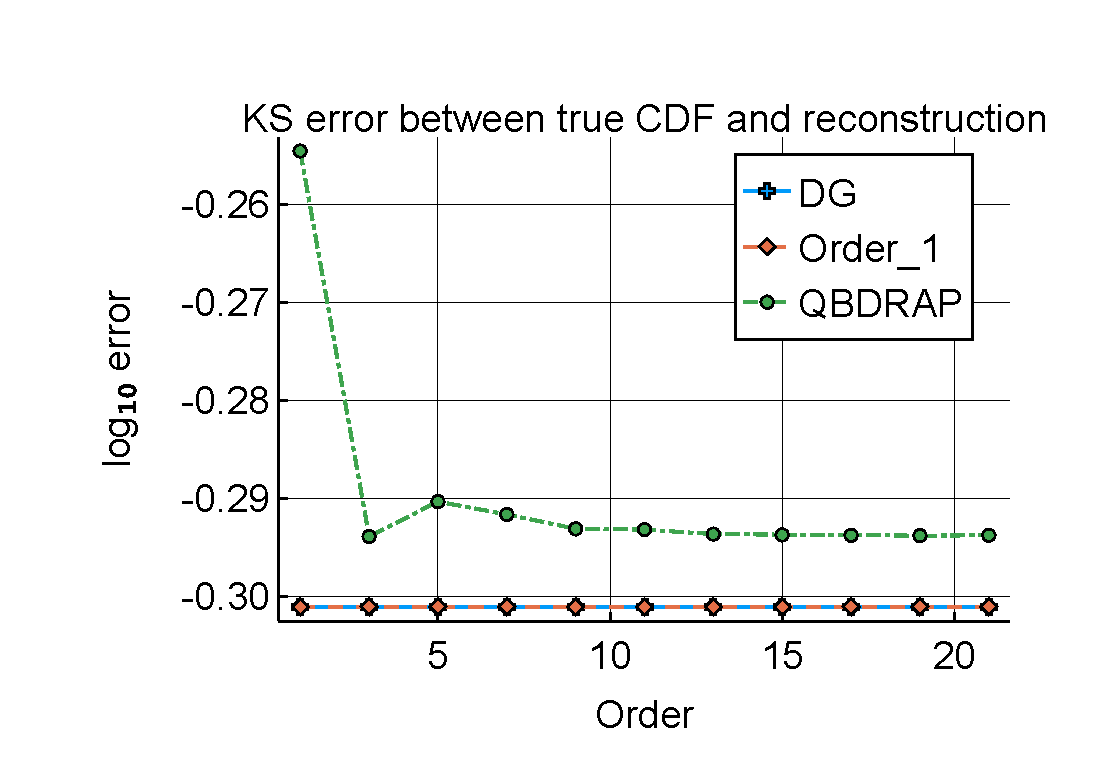
\includegraphics[width=0.5\textwidth,trim={1.25cm 0.8cm 0.25cm 1.25cm},clip]{chapter5/figs/comp/fun1/meshs_ks_error_formatted.pdf}%
	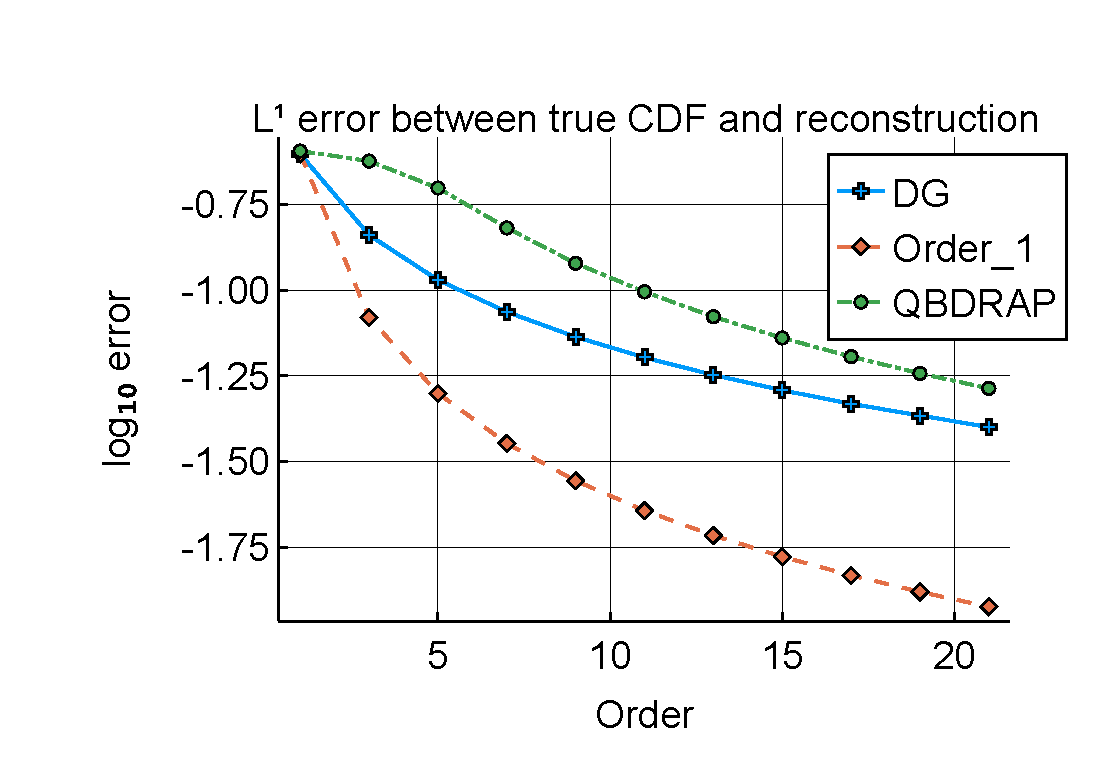
\includegraphics[width=0.5\textwidth,trim={1.25cm 0.8cm 0.25cm 1.25cm},clip]{chapter5/figs/comp/fun1/meshs_l1_cdf_error_formatted.pdf}
	\caption{KS error between the true CDF, \(1(x\geq 0.5)\), and the approximations (left) and \(L^1\) error between the true CDF and the approximations for the DG method (blue solid line with crosses), uniformisation method (orange dashed line with diamonds) and QBD-RAP method (green dash-dotted line with circles).}
	\label{fig: fun 1 comp} 
\end{figure}

In Figure~\ref{fig: pdf comp fun 1} we plot the approximated CDFs for the DG, uniformisation and QBD-RAP methods alonside the true CDF. The DG method displays undesireable fetures for an approximation to a CDF -- it is not monotonically increasing, at some points it is negative and at some points it is above 1. On the other hand, although the QBD-RAP method converges slowest, it displays good properties in that it results in a monotonically increasing CDF, starting at 0 and ending at 1. 
\begin{figure}
	\centering
	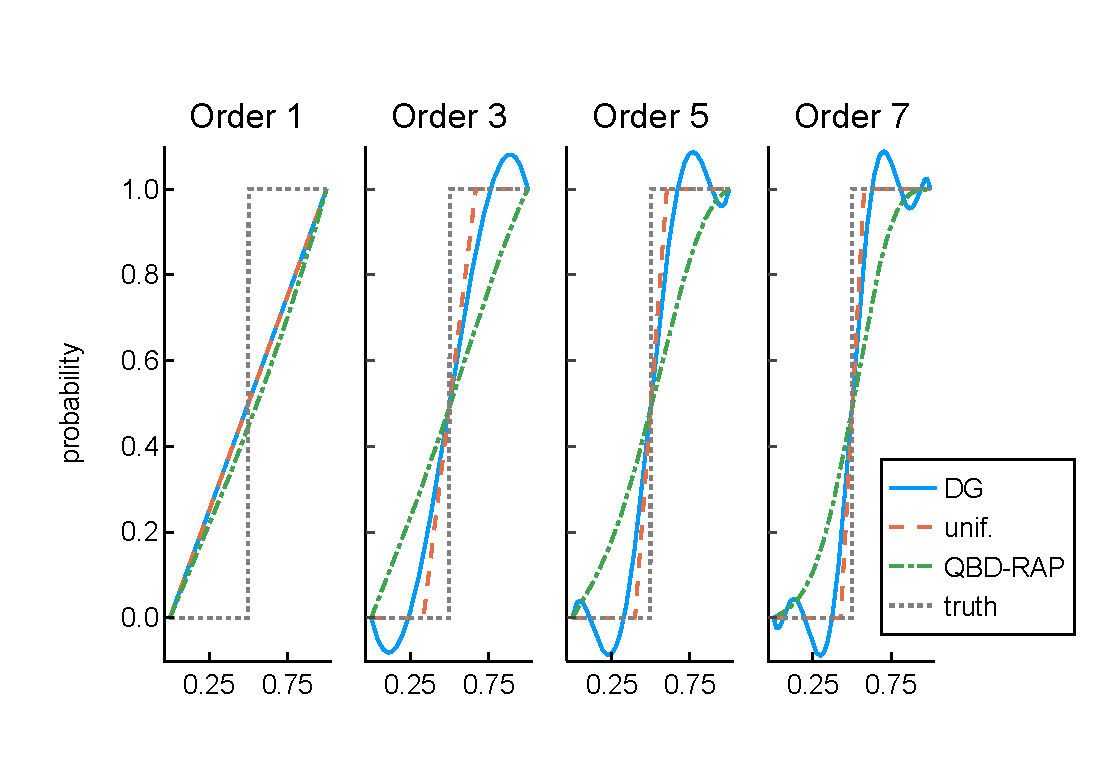
\includegraphics[width=\textwidth]{chapter5/figs/comp/fun1/cdfs_formatted.pdf}
	\caption{Reconstructed CDFs using the DG (blue solid line), uniformisation (orange dashed line) and QBD-RAP (green dot-dashed line) methods. The true distribution function is \(1(x\geq 0.5)\) (grey dotted line).}
	\label{fig: pdf comp fun 1}
\end{figure} 

Now consider approximaing the initial distribution with PDF \(1(x\leq 0.5)\). Figure~\ref{fig: fun 2 comp} plots the KS error (left) and \(L^2\) error between the true and approximate PDFs (right). Figure~\ref{fig: fun 2 comp} suggests that all methods converge at a similar rate for this problem. Once again, the QBD-RAP method performs worst, the uniformisation method second, and the DG method the best. However, once again the DG method exhibits undesireable properties -- the approximation to the CDF is, at some points above 1, is not monotonic, though these violations are not as severe in this case as they were for the case above. 
\begin{figure}
	\centering
	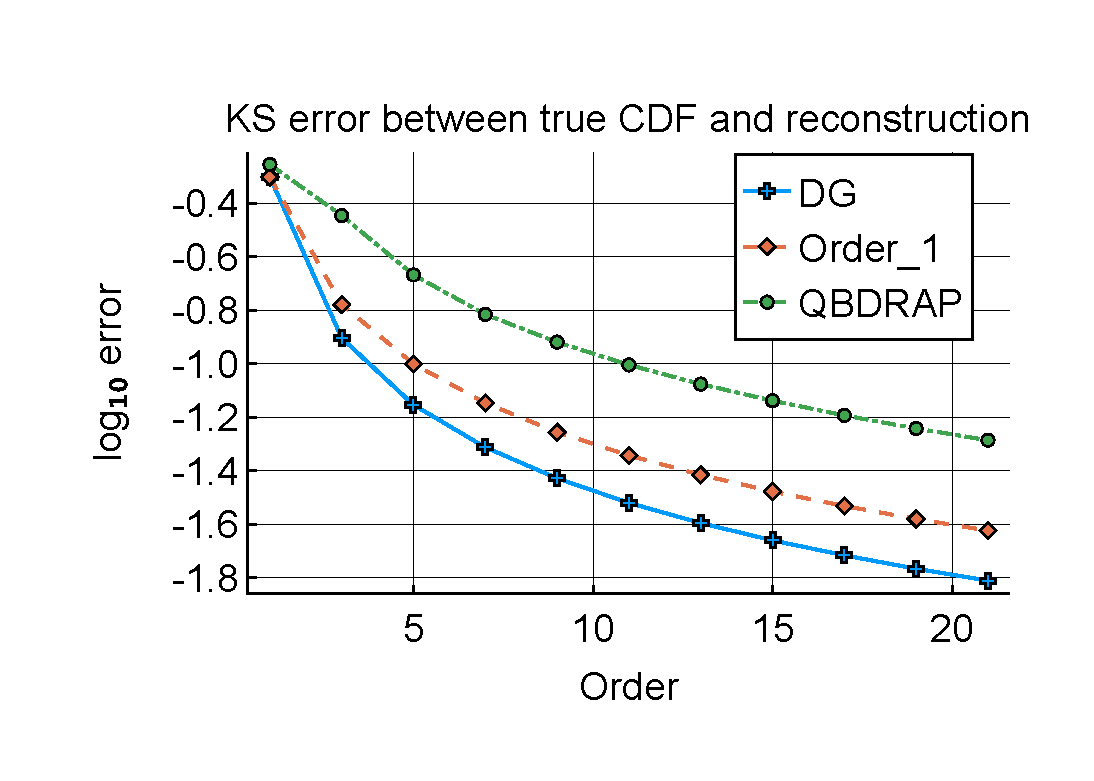
\includegraphics[width=0.5\textwidth,trim={1.25cm 0.8cm 0.25cm 1.25cm},clip]{chapter5/figs/comp/fun2/meshs_ks_error_formatted.pdf}%
	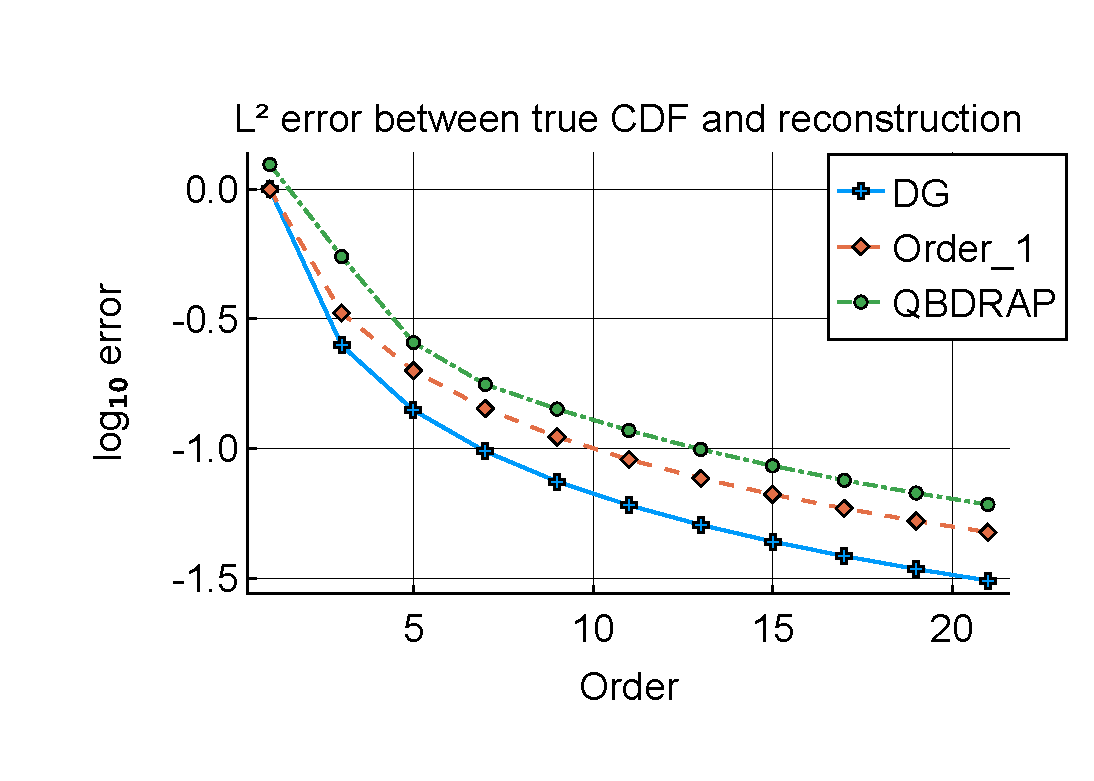
\includegraphics[width=0.5\textwidth,trim={1.25cm 0.8cm 0.25cm 1.25cm},clip]{chapter5/figs/comp/fun2/meshs_l2_pdf_error_formatted.pdf}
	\caption{KS error between the true CDF and the approximations (left) and \(L^2\) error between the true PDF, \(1(x\geq 0.5)\), and the approximations for the DG method (blue solid line with crosses), uniformisation method (orange dashed line with diamonds) and QBD-RAP method (green dash-dotted line with circles).}
	\label{fig: fun 2 comp} 
\end{figure}

So far we have considered two problems which exhibit discontinuities. At the other extreme we now consider an initial distribution with density \(-6z^2+6x\). In Figure~\ref{fig: fun 6 comp} we plot the KS error and the \(L^2\) error between the true and approximated PDF. Since the DG method projects the initial condition onto a polynomial basis, then, for an order 3 approximation and above, the DG method can theoretically approximate the initial condition exactly. This is reflected in Figure~\ref{fig: fun 6 comp}, where the blue curve drops sharply from 1-3, then plateaus. Due to numerical integration errors, for example in the evaluation of the integral in the \(L^2\) norm, and due to machine arithmetic, the errors for the DG scheme are not 0. Regarding the other two methods, they too appear to be convergent at approximately the same rate, with the uniformisation method perform better for the KS error, but very similarly in terms of the \(L^2\) error. 
\begin{figure}
	\centering
	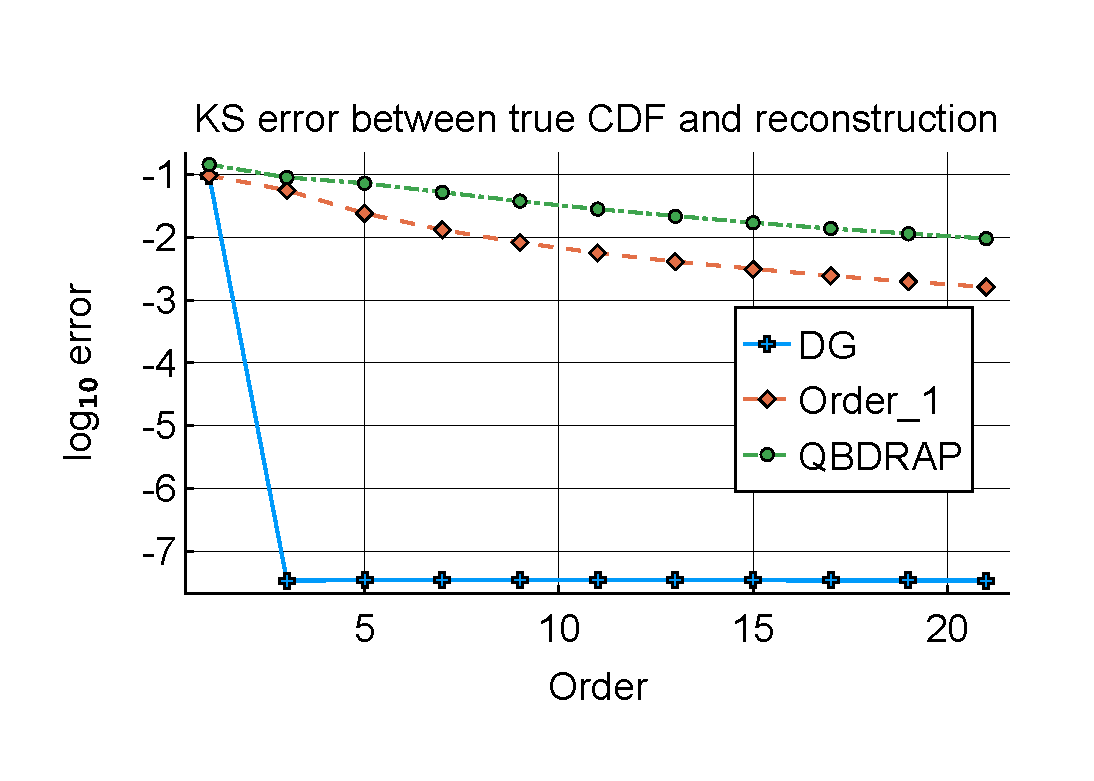
\includegraphics[width=0.5\textwidth,trim={1.25cm 0.8cm 0.25cm 1.25cm},clip]{chapter5/figs/comp/fun6/meshs_ks_error_formatted.pdf}%
	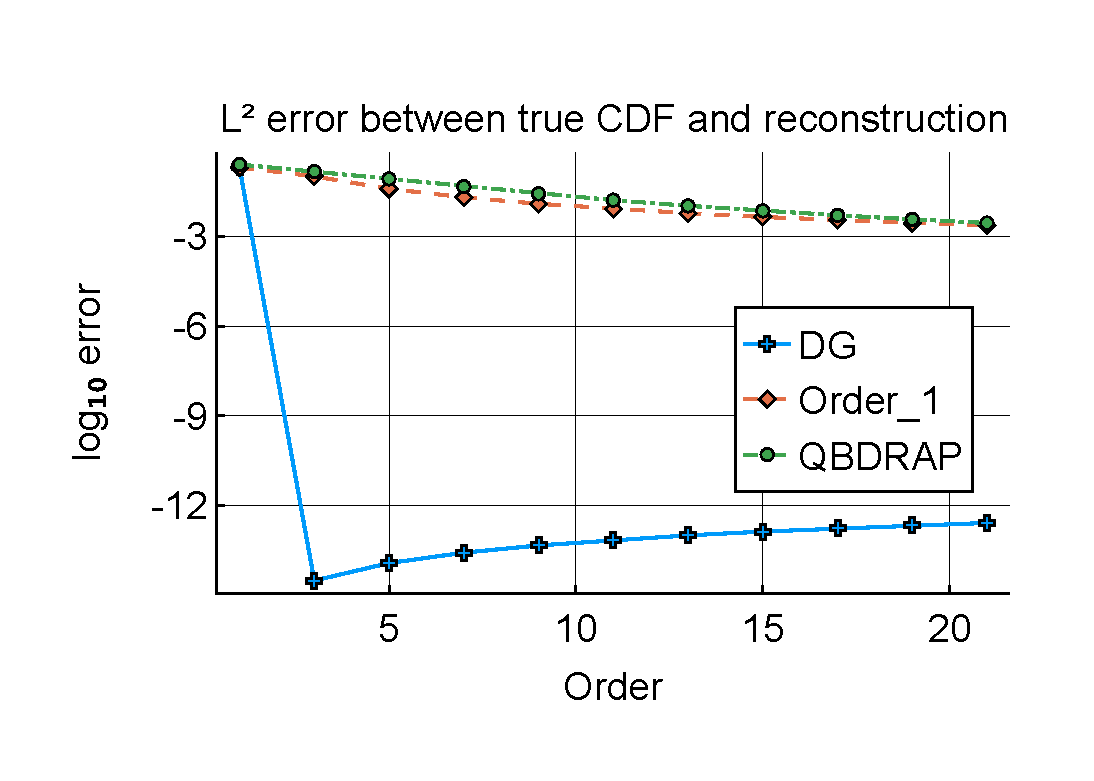
\includegraphics[width=0.5\textwidth,trim={1.25cm 0.8cm 0.25cm 1.25cm},clip]{chapter5/figs/comp/fun6/meshs_l2_pdf_error_formatted.pdf}
	\caption{KS error between the true CDF and the approximations (left) and \(L^2\) error between the true PDF, \(-6z^2+6x\), and the approximations for the DG method (blue solid line with crosses), uniformisation method (orange dashed line with diamonds) and QBD-RAP method (green dash-dotted line with circles).}
	\label{fig: fun 6 comp} 
\end{figure}

Consider now the initial distribution with PDF \(cos(4\pi(x+0.5))+1\). Figure~\ref{fig: fun 9 comp} shows the errors. Both the KS error (left) and \(L^2\) norm between the true and approximated PDFs tell a similar story. For sufficiently high order, the DG method approximates the inital condition very well. The uniformisation method performs second best, while the QBD-RAP method is slowest to converge. 
\begin{figure}
	\centering
	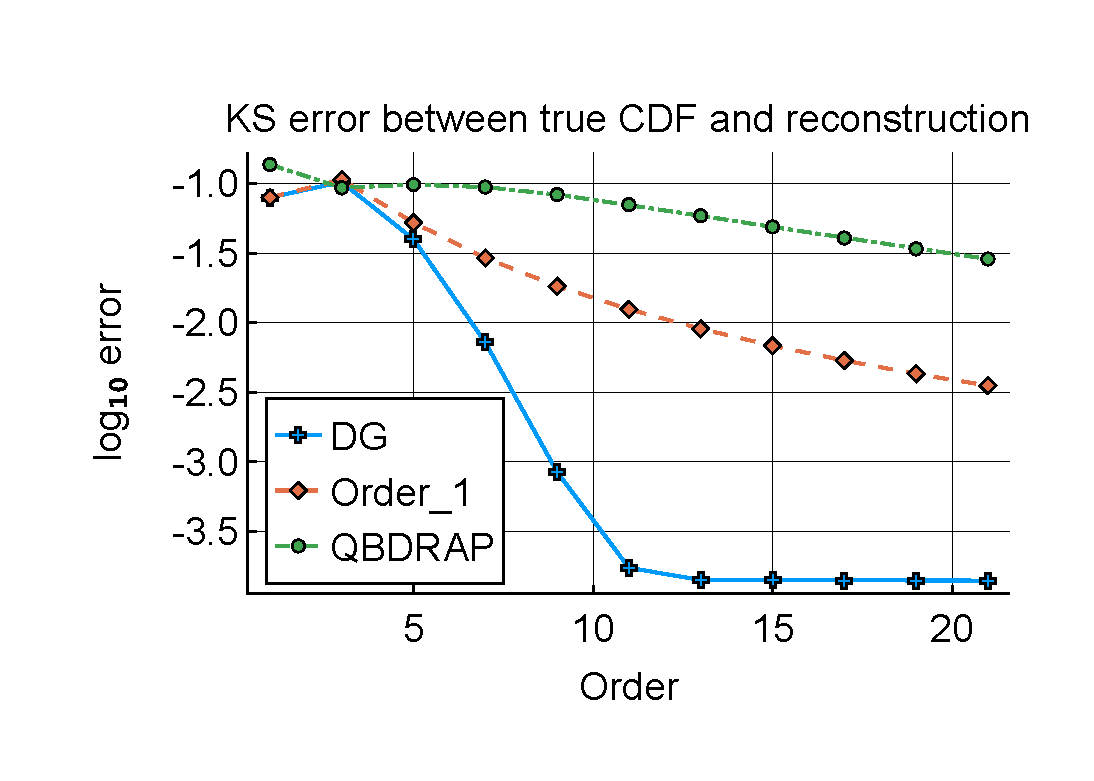
\includegraphics[width=0.5\textwidth,trim={1.25cm 0.8cm 0.25cm 1.25cm},clip]{chapter5/figs/comp/fun9/meshs_ks_error_formatted.pdf}%
	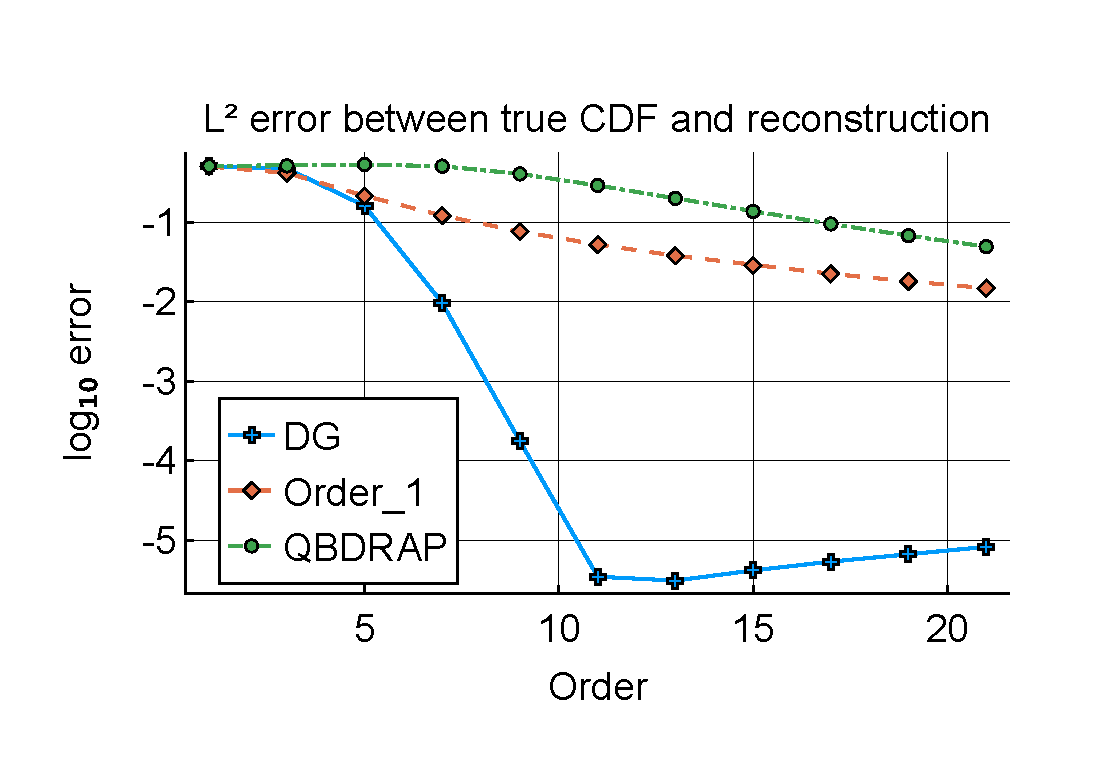
\includegraphics[width=0.5\textwidth,trim={1.25cm 0.8cm 0.25cm 1.25cm},clip]{chapter5/figs/comp/fun9/meshs_l2_pdf_error_formatted.pdf}
	\caption{KS error between the true CDF and the approximations (left) and \(L^2\) error between the true PDF, \(cos(4\pi(x+0.5))+1\), and the approximations for the DG method (blue solid line with crosses), uniformisation method (orange dashed line with diamonds) and QBD-RAP method (green dash-dotted line with circles).}
	\label{fig: fun 9 comp} 
\end{figure}
 
\FloatBarrier

\section{Travelling wave}
Here we investigate the performance the different schemes for approximating transient distributions of one-dimensional travelling wave problems with varying initial conditions. Consider a (trivial) fluid queue with one phase, generator \(\bs T=[0]\) and rate \(c=1\). The PDE (if/when it exists) which describes this system is 
\[\cfrac{\partial}{\partial t} f(x,t) = -\cfrac{\partial}{\partial x} f(x,t),\]
where \(f(x,t)\) is the density at time \(t\). Given an initial condition, \(f(x,0)\), solutions to this problem are given by 
\[f(x,t) = f(x-t,0)\]
so the solution at time \(t\) is just a shift in the initial condition \(t\) units to the right. We suppose that the fluid queue is bounded, with a lower boundary \(x=0\) and upper boundary \(x=10\). 

We use the QBD-RAP, uniformisation and DG schemes to discretise the solution in space. We discretise the interval \([0,10]\) into \(10\) cell, each of width 1. We use \(10,001\) points to approximate the integrals which appear in the construction of the initial conditions, to approximate the integrals appearing in the error metrics, and also as a set of discrete points on which evaluate the CDFs to approximate the KS metric. We use the SSPRK4 method to integrate over time using a step size of \(0.005\), and we evolve the system until time \(t=4\). For the DG method we also implement the Generalise MUSCL (REF, appendix?) slope limiter to stabilise the integration. 

First consider the initial condition with PDF \(1(x<1)\) so the level of the fluid queue is uniformly distributed over the first cell. For the DG and uniformisation methods, the initial condition can be represented exatly, whereas, for the QBD-RAP method, it cannot. Thus, in this case, there is no discretisation error in constructing the initial conition for the DG and uniformisation methods. 



































